\subsection{Content Recommendation}
Content recommendations are generated from a single Python script. It was decided to go with a single script as certain techniques are shared between user and post recommendations. The script is modularised by using functions that enable code blocks to be re-used. Python list comprehension provides a succinct way to generate lists \cite{Python:ListComprehension}, and this syntax is used throughout implementation.

Before recommendations can be made, a database connection is established using the \emph{mysql.connector} library, ``a Python driver for communicating with MySQL servers'' \cite{MySQL:MySQLConnector}. This library contains a number of useful functions for database interactions. Recommendation generation only occurs if the attempt to connect to the database is successful, otherwise an error message is logged. This prevents erroneous system behaviour. To begin recommendations, all users are first retrieved from the database. To tailor recommendations to a specific user, user settings for how they want their recommendations to be generated are retrieved. Default settings are set for new users but these can be changed on the settings page. The settings retrieved are for recommendation preference (FOF, Explorer or Hybrid recommendations), the number of recommendations to generate, recommendation threshold (for vector similarity) and recommendation reputation. Figure \ref{fig:RecommendationSettings} shows how user settings are retrieved.


\begin{figure}[H]
\centering
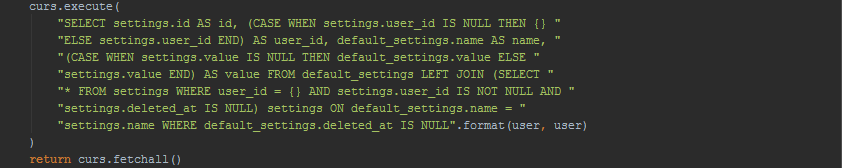
\includegraphics[width=\textwidth]{Images/Implementation/RecommendationSettings}
\caption{Query for user settings retrieval}
\label{fig:RecommendationSettings}
\end{figure}

Letting the user have control over these settings will allow them to fine-tune how they want to receive recommendations. Recommendations are generated using either FOF, Explorer or Hybrid users. The technique chosen for generation is dependent on the preference set by the user. To begin with, a query retrieving a count of the number of user recommendations already generated for the user is retrieved. New recommendations are only made if this count is less than the number of recommendations specified by the user. We will now look at how each of these techniques are implemented. Processes will be discussed for an individual user, who we will refer to as the recommendee, but each is repeated for all users stored in the database. The next two sections will look at how user and post recommendations are generated.

\subsubsection{Friend-of-a-Friend Recommendations}
FOF candidate recommendations are retrieved by first getting all users followed by the recommendee. These users are looped through, and for each of them the users they follow are collected and appended to a list. The recommendee is excluded from this list. Once this list has been generated, it is flattened to become a single list, which we will refer to as the \textit{fof\_users} list.

\paragraph{User} From this list, FOF user recommendations are chosen by converting the list to a \emph{Counter} object and picking the most common elements. The counter object was used for this purpose as it enables quick tallying \cite{Python:Counter} using the \textit{most\_common()} method. This function accepts a parameter value for the number of common elements to be returned, and by setting a value for it we can ensure that only the number of required recommendations for the recommendee are returned. Use of the Counter object is given below:

\begin{lstlisting}[language=python]
	fof_users = Counter(fof_users).most_common(num_recommendations)
\end{lstlisting}

Reasoning for not using cosine similarity between candidate recommendations and the recommendee are given in Chapter \ref{Chapter:Design}.

\paragraph{Post} Using the same technique for post recommendations, the users in the \textit{fof\_users} list are looped through, retrieving the posts made by each of the  users. For a post to suffice as a candidate recommendation for the recommendee, its reputation is compared with the reputation threshold set by the recommendee. If the reputation of the post exceeds the threshold, it is returned as one of the posts in the list of recommendations for the recommendee. Performing this check ensures again that recommendations being made are tailored to the recommendee's preferences.

\begin{figure}[H]
\centering
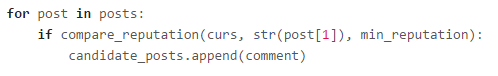
\includegraphics[width=\textwidth]{Images/Implementation/FOFPostReputation}
\caption{Code for assessing the reputation of a candidate post recommendation}
\label{fig:FOFPostReputation}
\end{figure} 

\subsubsection{Explorer Recommendations}
Explorer recommendations make use of the recommendee's `tag count vector', which is a vector representing the number of posts the recommendee has made in each of the available tags. The vector is generated by first creating a zero-filled list which has a length equal to the number of tags currently stored. Each entry in the list is a (TagID, Count) tuple. This list, which we shall refer to as the \emph{recommendee\_vector} is then sorted to determine the recommendee's favourite tags to post in. Candidate recommendations are retrieved from these tags. Currently, there is no cap on the number of tags looked at, but a cap on the number of `favourite tags' can be set once the system grows beyond what is considered small. The recommendee's favourite tags are looped through, retrieving other users posting in the same tag. This is shown in Figure \ref{fig:ExplorerFavouriteTags}.

\begin{figure}[H]
\centering
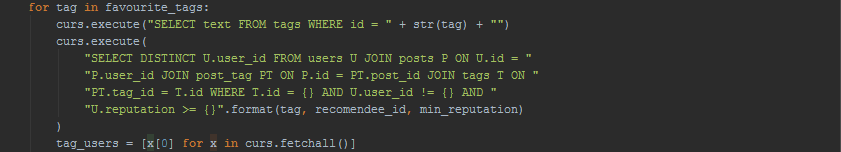
\includegraphics[width=\textwidth]{Images/Implementation/ExplorerFavouriteTags}
\caption{Code for retrieving users who post in the recommendee's preferred tags}
\label{fig:ExplorerFavouriteTags}
\end{figure}

\paragraph{User} Explorer user recommendations are assessed based on the similarity between a tag user (user also posting in one of the recommendee's preferred tags) and the recommendee. Similarity is measured using cosine similarity. SciPy provides a number of distance computation functions, one of which is the cosine distance. This is used to measure the distance between the vector generated for the tag user and the recommendee's vector. To get similarity from this, the result of this measurement is subtracted from one.

\begin{figure}[H]
\centering
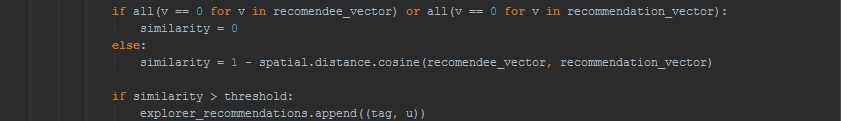
\includegraphics[width=\textwidth]{Images/Implementation/ExplorerSimilarity}
\caption{Measuring similarity between users for Explorer recommendations}
\label{fig:ExplorerSimilarity}
\end{figure}

\noindent In Figure \ref{fig:ExplorerSimilarity}, we see that we need to account for a user vector containing all zeros. This is possible for new or existing users who have made no posts. To handle such a situation, similarity is only measured if neither of the two user vectors contain only zeros. Once similarity is measured, it is compared with the threshold for similarity set by the user. Only users with a similarity that exceeds this threshold are given as recommendations. Before the set of user recommendations is returned, its length is compared with the number of recommendations needed to provide only the required number of recommendations. 

\paragraph{Post} Similarly to post recommendations generated using the FOF technique, posts made by each of the tag users are retrieved. Only those exceeding the reputation set by the recommendee are given as recommendations. Akin to user recommendations, only the number of required recommendations are returned.

\subsubsection{Hybrid Recommendations}
Hybrid recommendations are generated by finding the intersection between the recommendations made using the FOF and Explorer recommendation methods. The Python Standard Library provides a \textit{sets} module, which can create a set of unordered, unique elements from a list \cite{Python:Sets}. Using this module, it is possible to convert the lists returned from each of the recommendation methods to sets and find the intersection between the two. We can see this in Figure \ref{fig:HybridRecommendations}.

\begin{figure}[H]
\centering
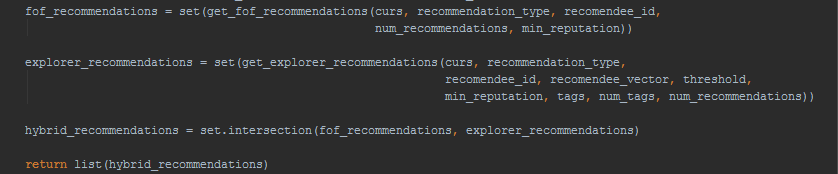
\includegraphics[width=\textwidth]{Images/Implementation/HybridRecommendations}
\caption{Generation of hybrid recommendations}
\label{fig:HybridRecommendations}
\end{figure}

\subsubsection{Default Recommendations}
In the event that all previous methods for generating recommendations fail, the script reverts to a default method that will generate generic recommendations for the recommendee. 

\paragraph{User} Default user recommendations will consist of users with the highest reputation in the system. To further filter this, only users with a reputation greater than the minimum reputation set by the user are returned.

\begin{figure}[H]
\centering
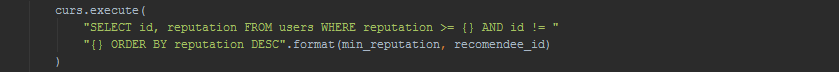
\includegraphics[width=\textwidth]{Images/Implementation/DefaultUsers}
\caption{Query for selecting most reputable users}
\label{fig:DefaultUsers}
\end{figure}

\paragraph{Post}
Similarly to users, default post recommendations are made based off the most reputable posts in the system.

\begin{figure}[H]
\centering
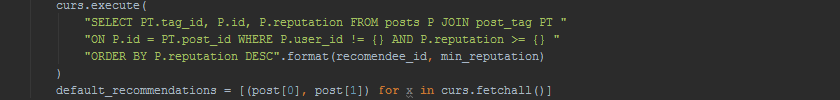
\includegraphics[width=\textwidth]{Images/Implementation/DefaultPosts}
\caption{Query for selecting most reputable posts}
\label{fig:DefaultPosts}
\end{figure}

\subsubsection{Cleaning and Saving Recommendations}
Once recommendations have been generated, they need to be cleaned. The first step in cleaning involves removing any recommendations the recommendee has not responded to. In addition to this, cleaning user recommendations consists of:
\begin{itemize}
\item Removing blocked users
\item Removing users the recommendee already follows
\item Removing the recommendee themselves
\end{itemize}

\noindent Cleaning post recommendations consists of:
\begin{itemize}
\item Removing posts made by users the recommendee has blocked
\item Removing posts the recommendee has voted on and therefore has already seen
\end{itemize}

In the case of cleaning post recommendations, posts made by the recommendee are not removed as all queries involving candidate post recommendations omit posts made by the recommendee.

Once recommendations have been cleaned, new recommendations are inserted into the relevant table. After storing the recommendations, changes made to the database must be committed using the \textit{commit()} function on the MySQL connection object.